% Main editable LaTeX source. Compile with Tectonic or latexmk.
% Data tables and the vector figure are prepared by ../build_report.py.
% Set encoding before IEEEtran initializes its Times family. This also
% prevents a TU/ptm font fallback when compiling with XeTeX/Tectonic.
\RequirePackage[T1]{fontenc}
\documentclass[conference,a4paper]{IEEEtran}
\usepackage{cite}
\usepackage{amsmath,amssymb}
\usepackage{booktabs}
\usepackage{balance}
\usepackage{graphicx}
\usepackage{url}
\usepackage[hidelinks]{hyperref}
\graphicspath{{assets/}}
% Generated from validated recorded measurements; do not edit.
\newcommand{\FKMaxPosition}{$4.429243\times 10^{-14}$}
\newcommand{\FKMaxOrientation}{$1.032631\times 10^{-13}$}
\newcommand{\IKMaxPosition}{$9.847942\times 10^{-6}$}
\newcommand{\IKMaxOrientation}{$7.038121\times 10^{-5}$}


\newcommand{\Rot}{\mathbf{R}}
\newcommand{\pos}{\mathbf{p}}
\newcommand{\q}{\mathbf{q}}
\newcommand{\Identity}{\mathbf{I}}
\newcommand{\SO}{\operatorname{SO}}
\newcommand{\Log}{\operatorname{Log}}
\newcommand{\clip}{\operatorname{clip}}

\title{Modified Denavit--Hartenberg Modeling and Numerical
Inverse Kinematics of the Open Duck Mini Robot}
% No student name or ID has been supplied. Replace the course-only block
% below with \IEEEauthorblockN{Your name} and an appropriate affiliation
% block when personal identification is required by the course.
\author{\IEEEauthorblockA{ROSE5710: Fundamental Robotics and Systems\\
Assignment 1: Kinematics, First Term 2026--2027}}

\begin{document}
\maketitle

\begin{abstract}
This report develops modified Denavit--Hartenberg models for the five-joint
left and right legs and the four-joint head--neck chain of the Open Duck
Mini robot. Joint directions and fixed site transforms are derived from
the supplied geometry and checked against the distributed MuJoCo model.
An inverse-kinematics solver combines a weighted position--orientation
objective with central finite differences, a fixed gradient-descent step,
and projection onto joint limits. Forward kinematics is evaluated at
300 seeded random configurations. Inverse kinematics is evaluated at
1,515 chain poses over five complete trajectory cycles. Every recorded
position and orientation error satisfies the assignment tolerances.
The measurements establish numerical agreement with the supplied
kinematic model; they do not constitute physical calibration or dynamic
tracking experiments.
\end{abstract}

\begin{IEEEkeywords}
Bipedal robots, forward kinematics, modified Denavit--Hartenberg
parameters, numerical inverse kinematics, MuJoCo.
\end{IEEEkeywords}

\section{Introduction}
The assignment requires analytical forward kinematics (FK) and numerical
inverse kinematics (IK) for two legs and a head--neck chain
\cite{assignment}. The model must reproduce both site position and
orientation, including the final fixed transform from the last joint to
the foot or head site. The distributed Open Duck Mini XML model supplies
the independent reference geometry \cite{open_duck}; MuJoCo computes its
reference body and site poses \cite{mujoco}.

The report gives the coordinate convention, all three modified
Denavit--Hartenberg (MDH) tables and joint signs, the required optimization
algorithm, and the measured FK/IK comparisons. Particular care is taken
with mirrored joint directions, offsets along parallel axes, and the
distinction between a solver stopping condition and independent acceptance
against the reference model.

\section{Modified Denavit--Hartenberg Model}
\subsection{Coordinate and transform conventions}
Column vectors are used. The homogeneous transform
${}^{i-1}\mathbf{T}_i$ maps coordinates from frame $i$ to frame $i-1$.
For row $i$, the prescribed MDH order is
\begin{equation}
\mathbf{A}_i
=\mathbf{R}_x(\alpha_{i-1})\mathbf{T}_x(a_{i-1})
 \mathbf{R}_z(\theta_i)\mathbf{T}_z(d_i).
\label{eq:mdh}
\end{equation}
Unlike the standard DH indexing, the revolute axis of joint $i$ is
$z_i$ in this convention; $x_{i-1}$ follows a common normal to
$z_{i-1}$ and $z_i$. Intersecting axes permit a zero common-normal
length. Writing $c_\theta=\cos\theta_i$, $s_\theta=\sin\theta_i$,
$c_\alpha=\cos\alpha_{i-1}$, and $s_\alpha=\sin\alpha_{i-1}$ gives
\begin{equation}
\mathbf{A}_i=\begin{bmatrix}
c_\theta & -s_\theta & 0 & a_{i-1}\\
c_\alpha s_\theta & c_\alpha c_\theta & -s_\alpha & -d_i s_\alpha\\
s_\alpha s_\theta & s_\alpha c_\theta & c_\alpha & d_i c_\alpha\\
0&0&0&1
\end{bmatrix}.
\label{eq:matrix}
\end{equation}
For a chain with $n$ actuated joints and one fixed site row,
\begin{align}
\theta_i&=s_iq_i+\theta_i^0,\quad i=1,\ldots,n,\label{eq:sign}\\
{}^B\mathbf{T}_S(\q)&={}^B\mathbf{T}_0
 \prod_{i=1}^{n+1}\mathbf{A}_i,\label{eq:fk}
\end{align}
where row $n+1$ contains no joint variable. The factors are accumulated
from left to right in increasing row order. All distances in the tables
are in metres and angles are in radians. The code stores rows as
$[\alpha,a,\theta^0,d]$; the printed tables use the assignment order
$[\alpha,a,d,\theta]$.

\subsection{Left and right leg chains}
Define the base-to-yaw planar distance and angle by
\begin{align}
r&=\sqrt{0.019^2+0.035^2}=0.03982461550348\ \mathrm{m},\\
\beta&=\operatorname{atan2}(19,35)=0.49734271634682.
\end{align}
The supplied base-to-frame-zero transforms are retained:
\begin{align}
{}^B\mathbf{T}_{0,L}&=\mathbf{R}_z(\pi/2+\beta),\\
{}^B\mathbf{T}_{0,R}&=\mathbf{R}_z(-\pi/2-\beta).
\end{align}
Here rotations are understood as homogeneous transforms with zero
translation. The signs relating MuJoCo joint coordinates to MDH angles
are
\begin{align}
\mathbf{s}_L&=[1,-1,-1,-1,-1]^{\mathsf T},\\
\mathbf{s}_R&=[1,-1,1,-1,-1]^{\mathsf T}.
\end{align}
Tables~\ref{tab:dh-left} and~\ref{tab:dh-right} give all joint and site
rows. At zero joint angles, both legs use the MDH directions
$z_1=+Z$, $z_2=+X$, and $z_3=z_4=z_5=+Y$. The first two MuJoCo
joint directions are $+Z$ and $-X$. The three pitch directions are
$(-Y,-Y,-Y)$ on the left and $(+Y,-Y,-Y)$ on the right. These
directions explain the different signs of the third joint.

\begin{table}[t]
\centering
\footnotesize
\setlength{\tabcolsep}{4pt}
\caption{Modified D--H parameters for the left leg. Lengths $a,d$ are in metres; angles $\alpha,\theta,q$ are in radians. The starred final row is the fixed site transform.}
\label{tab:dh-left}
\begin{tabular}{ccccc}
\toprule
$i$ & $\alpha_{i-1}$ & $a_{i-1}$ & $d_i$ & $\theta_i$ \\
\midrule
$1$ & $0$ & $r$ & $-0.0000741$ & $q_{1}-\beta$ \\
$2$ & $\pi/2$ & $0$ & $-0.01606$ & $-q_{2}+\pi/2$ \\
$3$ & $\pi/2$ & $0$ & $0.07415$ & $-q_{3}+\pi$ \\
$4$ & $0$ & $0.07865$ & $0$ & $-q_{4}$ \\
$5$ & $0$ & $0.07865$ & $-0.01975$ & $-q_{5}-\pi/2$ \\
$6^{*}$ & $\pi/2$ & $0.0005$ & $-0.036225$ & $0$ \\
\bottomrule
\end{tabular}
\end{table}

\begin{figure}[H]
\centering
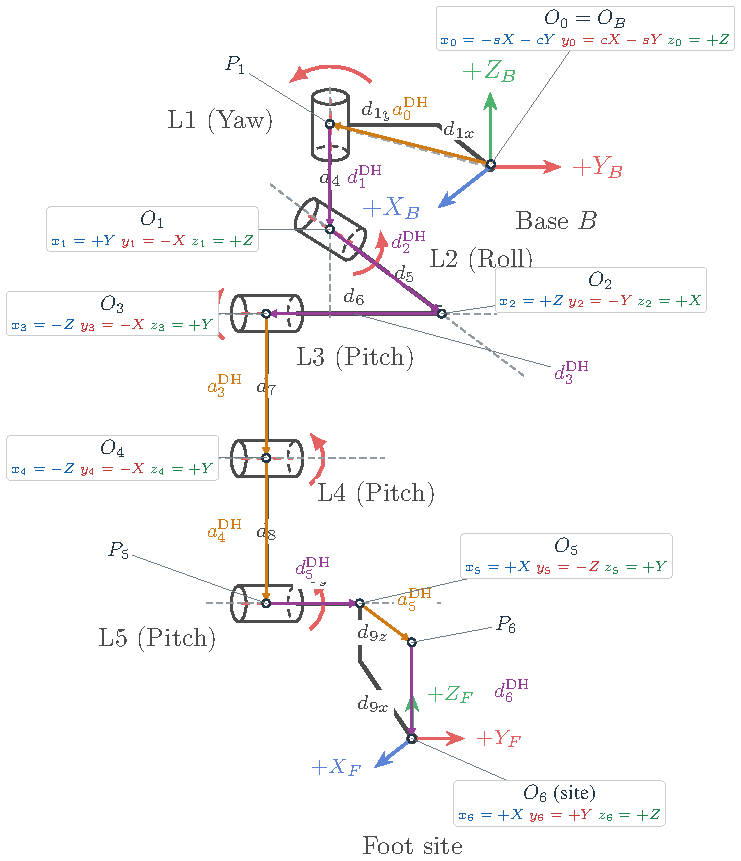
\includegraphics[width=\linewidth,height=128mm,keepaspectratio]{dh_right_annotated_panel.pdf}
\caption{\small Right leg: annotated assignment Fig.~3 \cite{assignment}. $O_i$: D-H origins; $P_i$: intermediate points. Orange: $a_{i-1}$; purple: $d_i$. Boxes give positive XYZ directions in $B$.}
\label{fig:dh-right}
\end{figure}
\begin{table}[H]
\centering
\small
\setlength{\tabcolsep}{4pt}
\caption{\small Right leg: D--H parameters (m, rad) and zero-pose axes in frame $B$.}
\label{tab:dh-right}
\medskip
\begin{minipage}[t]{0.54\linewidth}
\centering
\begin{tabular}{ccccc}
\toprule
$i$ & $\alpha_{i-1}$ & $a_{i-1}$ & $d_i$ & $\theta_i$ \\
\midrule
$1$ & $0$ & $r$ & $-0.0000741$ & $q_{1}+\pi+\beta$ \\
$2$ & $\pi/2$ & $0$ & $-0.01606$ & $-q_{2}+\pi/2$ \\
$3$ & $\pi/2$ & $0$ & $-0.07415$ & $q_{3}+\pi$ \\
$4$ & $0$ & $0.07865$ & $0$ & $-q_{4}$ \\
$5$ & $0$ & $0.07865$ & $0.01735$ & $-q_{5}-\pi/2$ \\
$6^{*}$ & $\pi/2$ & $0.0005$ & $-0.036225$ & $0$ \\
\bottomrule
\end{tabular}
\par\medskip
{\footnotesize\raggedright $^*$ Fixed foot site. The combined lateral pitch-axis offset is $17.35\,\mathrm{mm}$ on the right ($19.75\,\mathrm{mm}$ on the left).\par}
\end{minipage}\hfill
\begin{minipage}[t]{0.43\linewidth}
\centering
\setlength{\tabcolsep}{3pt}
\begin{tabular}{cccc}
\toprule
$i$ & $+x_i$ & $+y_i$ & $+z_i$ \\
\midrule
$0$ & $-sX-cY$ & $cX-sY$ & $+Z$ \\
$1$ & $+Y$ & $-X$ & $+Z$ \\
$2$ & $+Z$ & $-Y$ & $+X$ \\
$3$ & $-Z$ & $-X$ & $+Y$ \\
$4$ & $-Z$ & $-X$ & $+Y$ \\
$5$ & $+X$ & $-Z$ & $+Y$ \\
$6^{*}$ & $+X$ & $+Y$ & $+Z$ \\
\bottomrule
\end{tabular}
\par\medskip
{\footnotesize\raggedright $X,Y,Z$ are base-frame unit axes. $s=\sin\beta$, $c=\cos\beta$.\par}
\end{minipage}
\end{table}


The first two MDH origins are chosen at the yaw/roll and roll/pitch axis
intersections rather than at arbitrary CAD body origins. The effective
roll-axis height follows directly from the XML offsets:
\begin{equation}
45.9409-46.015=-0.0741\ \mathrm{mm}.
\end{equation}
Translations along the three parallel pitch axes commute with their
joint rotations and may be combined at a selected origin. This yields
the supplied final lateral distances of $19.75\ \mathrm{mm}$ on the
left and $17.35\ \mathrm{mm}$ on the right. A completely mirrored
table would therefore be incorrect. The final fixed row restores the
foot-site orientation, which is the identity in the zero pose.

\subsection{Head and neck chain}
The supplied neck anchor is already represented in the initial transform:
\begin{equation}
{}^B\mathbf{T}_{0,H}=\begin{bmatrix}
\Identity_3&\pos_c\\\mathbf{0}^{\mathsf T}&1
\end{bmatrix},\qquad
\pos_c=\begin{bmatrix}0.001\\0.01915\\0.0900009\end{bmatrix}\mathrm{m}.
\end{equation}
The four zero-pose joint axes are $[-Y,-Y,+Z,-X]$, matching the MuJoCo
positive directions, so $\mathbf{s}_H=[1,1,1,1]^{\mathsf T}$.
Table~\ref{tab:dh-head} contains the corresponding five rows.

\begin{table}[t]
\centering
\footnotesize
\setlength{\tabcolsep}{4pt}
\caption{Modified D--H parameters for the head. Lengths $a,d$ are in metres; angles $\alpha,\theta,q$ are in radians. The starred final row is the fixed site transform.}
\label{tab:dh-head}
\begin{tabular}{ccccc}
\toprule
$i$ & $\alpha_{i-1}$ & $a_{i-1}$ & $d_i$ & $\theta_i$ \\
\midrule
$1$ & $\pi/2$ & $0$ & $0$ & $q_{1}+\pi/2$ \\
$2$ & $0$ & $0.066$ & $0.01905$ & $q_{2}-\pi/2$ \\
$3$ & $-\pi/2$ & $0$ & $0.03785$ & $q_{3}+\pi/2$ \\
$4$ & $-\pi/2$ & $0$ & $-0.005$ & $q_{4}$ \\
$5^{*}$ & $\pi/2$ & $0$ & $0.04245$ & $-\pi/2$ \\
\bottomrule
\end{tabular}
\end{table}


The base-to-neck distance labelled $92.021\ \mathrm{mm}$ in the handout
is already contained in $\pos_c$ and is not added a second time. The
neck-to-head-pitch separation is $66\ \mathrm{mm}$. The effective
vertical separation from the head-pitch axis to the roll axis is
$37.85\ \mathrm{mm}$, and the net roll-axis offset is $5\ \mathrm{mm}$.

\subsection{Analytical zero-pose check}
Let $d_{1x},d_{1y},d_4,\ldots,d_{9z}$ denote the leg dimensions in
Fig.~2 of the handout, converted to metres. The MDH construction gives
\begin{align}
\pos_L(\mathbf{0})&=\begin{bmatrix}
-d_{1x}+d_5+d_{9x}\\d_{1y}+d_6-d_{9y}\\-d_4-d_7-d_8-d_{9z}
\end{bmatrix},\\
\pos_R(\mathbf{0})&=\begin{bmatrix}
-d_{1x}+d_5+d_{9x}\\-d_{1y}-d_6+d_{9y}\\-d_4-d_7-d_8-d_{9z}
\end{bmatrix}.
\end{align}
For the head dimensions in Fig.~4,
\begin{equation}
\pos_H(\mathbf{0})=\pos_c+[d_5,-d_3,d_2+d_4+d_6]^{\mathsf T}.
\end{equation}
The resulting site positions are listed in Table~\ref{tab:zero}, and
all three zero-pose site rotations are $\Identity_3$.

\begin{table}[t]
\caption{Analytical and XML zero-pose positions in the base frame.}
\label{tab:zero}
\centering\footnotesize
\begin{tabular}{lrrr}
\toprule
Site & $x$ [m] & $y$ [m] & $z$ [m]\\
\midrule
Left foot & $-0.03456$ & $0.08940$ & $-0.1935991$\\
Right foot & $-0.03456$ & $-0.09180$ & $-0.1935991$\\
Head & $0.00600$ & $0.00010$ & $0.2363009$\\
\bottomrule
\end{tabular}
\end{table}

\section{Numerical Inverse Kinematics}
\subsection{Position--orientation objective}
For target pose $(\pos_t,\Rot_t)$ and FK prediction
$(\pos(\q),\Rot(\q))$, define base-frame residuals
\begin{align}
\mathbf{e}_p(\q)&=\pos_t-\pos(\q),\\
\mathbf{e}_R(\q)&=\Log\!\left(\Rot_t\Rot(\q)^{\mathsf T}\right)^\vee.
\end{align}
Here $\Log$ is the principal rotation logarithm, and $\vee$ maps its
skew-symmetric matrix to a rotation vector. Its norm is the shortest
relative rotation angle, avoiding Euler-angle
subtraction. The required dimensionless cost is
\begin{equation}
E(\q)=\lVert s_p\mathbf{e}_p(\q)\rVert_2^2
       +\lVert\mathbf{e}_R(\q)\rVert_2^2,
\qquad s_p=10\ \mathrm{m}^{-1}.
\label{eq:cost}
\end{equation}
Candidate evaluations use FK only and do not modify MuJoCo state.

\subsection{Finite differences and bounded updates}
Let $\mathbf{u}_i$ be the $i$th coordinate basis vector and set
$h=10^{-6}\ \mathrm{rad}$. At iteration $k$, the gradient component is
approximated by
\begin{equation}
g_i^{(k)}=\frac{E(\q^{(k)}+h\mathbf{u}_i)-E(\q^{(k)}-h\mathbf{u}_i)}{2h}.
\label{eq:gradient}
\end{equation}
The fixed-step update is
\begin{equation}
\q^{(k+1)}=\clip\!\left(\q^{(k)}-0.1\mathbf{g}^{(k)},
                          \q_{\min},\q_{\max}\right),
\label{eq:update}
\end{equation}
with joint limits read from the XML model. The initial guess is the
current state of the selected chain. At most 5,000 iterations are allowed
per target, with termination when $E<10^{-8}$.

Since both terms in~\eqref{eq:cost} are nonnegative, the cost criterion
implies
\begin{equation}
\lVert\mathbf{e}_p^{\mathrm{FK}}\rVert_2<10^{-5}\ \mathrm{m},\qquad
\lVert\mathbf{e}_R^{\mathrm{FK}}\rVert_2<10^{-4}\ \mathrm{rad}.
\end{equation}
This statement bounds the FK-model residual. It does not guarantee that
fixed-step projected gradient descent converges before the iteration
limit. Final acceptance is therefore evaluated independently using the
MuJoCo site pose after the solved angles have been written to the model.

\subsection{Supplied task-space trajectories}
For phase $\phi\in[0,1]$, the foot displacements are
\begin{align}
\Delta\pos_L(\phi)&=0.020\sin^2(\pi\phi)(\mathbf{e}_x+\mathbf{e}_z),\\
\Delta\pos_R(\phi)&=0.020\cos^2(\pi\phi)(\mathbf{e}_x+\mathbf{e}_z),
\end{align}
in metres, with fixed starting orientations. The head follows a reachable
neck-centred arc. With $\gamma=0.1\sin^2(\pi\phi)$,
\begin{align}
\pos_{t,H}(\phi)&=\pos_c+\Rot_y(-\gamma)(\pos_{H,0}-\pos_c),\\
\Rot_{t,H}(\phi)&=\Rot_y(-\gamma)\Rot_{H,0}.
\end{align}
The bent-leg and head starting configurations are
\begin{align}
\q_{L,0}&=[0,0,-0.4,0.8,-0.4]^{\mathsf T},\\
\q_{R,0}&=[0,0,0.4,0.8,-0.4]^{\mathsf T},\\
\q_{H,0}&=[0.2,-0.4,0,0]^{\mathsf T}.
\end{align}
The base is fixed at a height of $0.19\ \mathrm{m}$. Subsequent targets
are warm-started from the previous solution, including across cycle
boundaries; the initial joint angles are not reset each cycle.

\balance
\section{Experimental Evaluation}
\subsection{Protocol and error measures}
Every comparison uses base-frame site poses. World-frame MuJoCo
transforms are converted by
\begin{equation}
{}^B\mathbf{T}_S^{\mathrm{MJ}}
=\left({}^W\mathbf{T}_B\right)^{-1}{}^W\mathbf{T}_S.
\end{equation}
For two poses $(\pos_a,\Rot_a)$ and $(\pos_b,\Rot_b)$, the reported errors
are
\begin{align}
\epsilon_p&=\lVert\pos_a-\pos_b\rVert_2,\\
\epsilon_R&=\big\lVert\Log(\Rot_a\Rot_b^{\mathsf T})^\vee\big\rVert_2.
\end{align}
FK is compared at 100 configurations per chain, with each joint sampled
uniformly within its limits and random seed zero used for each chain.
IK follows five complete cycles, each with 101 phase samples for each of
the three chains: 1,515 measured site poses in total.

The stored experiment used Python 3.11.18, NumPy 1.26.4, SciPy 1.14.1,
and MuJoCo 3.2.4. The FK, IK, and XML source fingerprints recorded in
the experiment manifest still match the current files. The existing
measurements are audited and reused for this typeset report; recompiling
the report does not rerun the simulation. Headless operation changes
only viewer rendering and its delay.

\subsection{Measured results}
Tables~\ref{tab:fk} and~\ref{tab:ik} report maxima over all stored samples.
The required FK limits are $\epsilon_p<10^{-6}\ \mathrm{m}$ and
$\epsilon_R<10^{-5}\ \mathrm{rad}$; the IK limits are
$\epsilon_p<10^{-5}\ \mathrm{m}$ and $\epsilon_R<10^{-4}\ \mathrm{rad}$.
Every recorded value is finite and satisfies its corresponding limit.
The largest FK position and orientation errors are \FKMaxPosition{}~m
and \FKMaxOrientation{}~rad, respectively. The corresponding largest IK
errors are \IKMaxPosition{}~m and \IKMaxOrientation{}~rad.

\begin{table}[H]
\centering
\small
\setlength{\tabcolsep}{10pt}
\caption{Measured FK errors over 300 random configurations. Maxima are computed independently for each chain.}
\label{tab:fk}
\medskip
\begin{tabular}{lccc}
\toprule
Chain & \shortstack{Max. position\\(m)} & \shortstack{Max. orientation\\(rad)} & Result \\
\midrule
Left leg & $8.455733\times 10^{-15}$ & $2.283510\times 10^{-14}$ & PASS \\
Right leg & $4.429498\times 10^{-14}$ & $2.375025\times 10^{-14}$ & PASS \\
Head & $6.572043\times 10^{-15}$ & $1.032631\times 10^{-13}$ & PASS \\
\bottomrule
\end{tabular}
\end{table}

\begin{table}[H]
\centering
\small
\setlength{\tabcolsep}{10pt}
\caption{Measured IK errors over 1,515 trajectory poses. Maxima are computed independently for each chain.}
\label{tab:ik}
\medskip
\begin{tabular}{lccc}
\toprule
Chain & \shortstack{Max. position\\(m)} & \shortstack{Max. orientation\\(rad)} & Result \\
\midrule
Left leg & $9.847942\times 10^{-6}$ & $6.846493\times 10^{-5}$ & PASS \\
Right leg & $9.844913\times 10^{-6}$ & $7.038121\times 10^{-5}$ & PASS \\
Head & $8.393151\times 10^{-6}$ & $6.773237\times 10^{-5}$ & PASS \\
\bottomrule
\end{tabular}
\end{table}


\begin{figure*}[t]
\centering
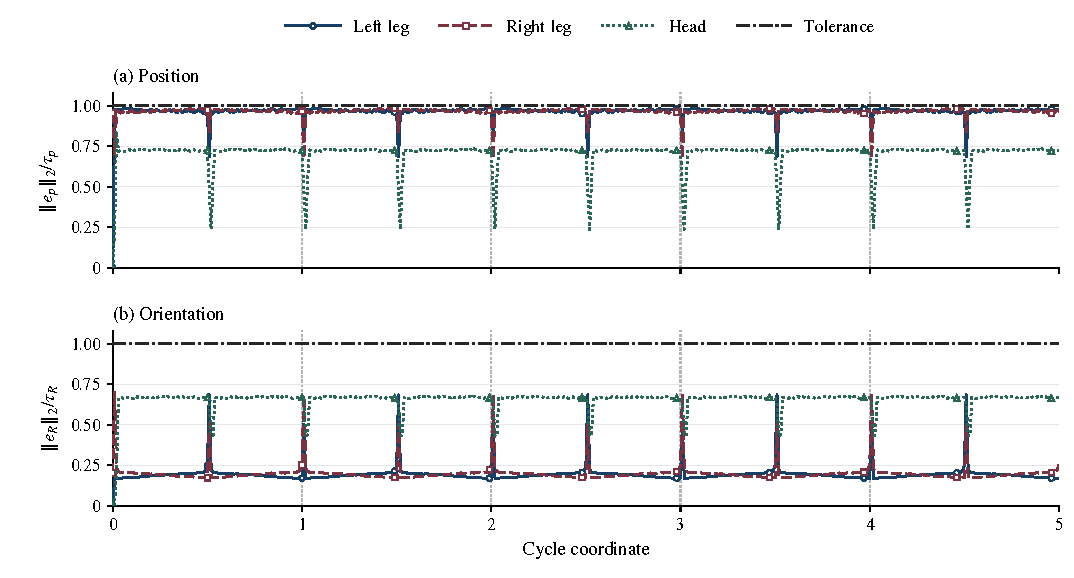
\includegraphics[width=\textwidth]{ik_error_plot.pdf}
\caption{All measured IK errors, normalized by their acceptance limits:
$\tau_p=10^{-5}\ \mathrm{m}$ for position and $\tau_R=10^{-4}\ \mathrm{rad}$ for
orientation. Each curve contains all 505 targets for one chain, including
the initial values; the full comparison contains 1,515 chain poses.
An ordinate of one is the acceptance boundary. Vertical lines separate
the five cycles. Line styles and markers distinguish the chains in
monochrome. No smoothing or resampling is applied; line segments connect
adjacent measurements.}
\label{fig:ik}
\end{figure*}

Figure~\ref{fig:ik} shows the full chronological record without dropping
initial or boundary samples. Errors near the position threshold are
consistent with terminating at the specified weighted-cost criterion;
the solver is not required to optimize each target to machine precision.
The largest position error remains below the required limit.

\subsection{Regression checks and scope}
Six regression test cases additionally cover XML-based zero poses,
random configurations under a translated and rotated floating base,
the metric weights and relative-rotation angle in the objective,
an unchanged target pose, nearby reachable IK targets, and projection
onto joint limits. The IK checks also verify that the base and unselected
chains are preserved.

The comparison loops update site poses with MuJoCo's
\texttt{mj\_forward} routine, without dynamic stepping. The very small
FK errors quantify agreement with the numerical XML model; they do not
measure physical link calibration. The random configurations do not
exhaust the joint domain. The experiment does not evaluate contact
stability, real-robot dynamics, or arbitrary-target IK convergence.

\section{Conclusion}
The derived MDH chains reproduce all three sites of the supplied robot
model, including mirrored joint signs and the fixed terminal transforms.
The prescribed central-difference, fixed-step IK method satisfies all
position and orientation tolerances over the complete supplied trajectory
test. The three MDH tables, measured records, source fingerprints, vector
figure, and editable LaTeX sources provide a reproducible submission.

\appendices
\section{Reproduction}
The repository includes a pinned Python 3.11 environment, FK and IK entry
points, and six regression test cases. Full command lines for the complete
headless comparison and JSON exports are included in the supplied README.

The report builder prepares tables from the measured JSON files and
compiles the paper with a LaTeX engine. Its manifest records the engine
version, compile status, and input fingerprints. The source package
contains full command lines, generated tables, a bibliography, and the
vector figure, so the document can also be compiled independently.

\bibliographystyle{IEEEtran}
\bibliography{references}
\end{document}
